\PassOptionsToPackage{offset}{pdfpcnotes}

\documentclass[
% auto_overview,
auto_sections,
% show_durations,
% monitor_progress,
% draft
]{mannbeamer}

\setkeys{Gin}{draft=false}

\usepackage[utf8]{inputenc}
\usepackage[T1]{fontenc}

\usepackage{default}

\usetikzlibrary{arrows,arrows.meta,calc,positioning,shapes,decorations.pathreplacing,decorations.markings}

\setbeamertemplate{caption}{\raggedright\insertcaption\par}

\usepackage[backend=biber,maxcitenames=1,doi=false,isbn=false,url=false]{biblatex}
\addbibresource{thesis.bib}

% Complex arrays with diagonal headers
\usepackage{booktabs}
\usepackage{adjustbox}
\usepackage{array}
\usepackage{multirow}

\usepackage{multimedia}

\usepackage{amsmath}

\usepackage{qrcode}

\let\vec\mathbf

% Seems to work. But I'm really not sure.
\AtDataInput{%
  \stepcounter{citations}
}

\DeclareCiteCommand{\citejournal}
  {\usebibmacro{prenote}}
  {\usebibmacro{citeindex}\usebibmacro{journal}}
  {\multicitedelim}
  {\usebibmacro{postnote}}
\newcommand{\mycite}[2][\tiny]{\stepcounter{citations}{#1\citeauthor{#2} \citeyear{#2} - \citejournal{#2}}}
\newcommand{\mysmallcite}[2][\tiny]{\stepcounter{citations}{#1\citeauthor{#2} (\citeyear{#2})}}

\graphicspath{{annexes/}{annexes_slides/}}

\titleheader{
 \includegraphics[height=1.5cm]{logos/IRIT}
 \hfill
 \includegraphics[height=1.5cm]{logos/REVA}
 \hfill
 \includegraphics[height=1.5cm]{logos/UTMP}
}
\title{Splinoids project outline}
\author{GODIN-DUBOIS Kevin}
% \formation{Background}
% \date{March 31st, 2020}
\titlemisc{
 \begin{tabular}{l}
  Generated on \today \\
  Perma-link: \href{https://github.com/kgd-al/Splinoids/blob/master/doc/outline.pdf}{kgd-al@github}
 \end{tabular}
}
\duration{8}
\notessize{30}

\begin{document}

\dotitlepage

\newcommand{\splinoid}[2][]{\includegraphics[draft=false,#1]{annexes/splinoids_#2.png}}
\section{Splinoids}

\begin{frame}[ok]
 \frametitle{Spline + Boids}
 \centering
 \begin{minipage}{.49\textwidth}
  \splinoid[width=\textwidth, height=.8\textheight, keepaspectratio]{large}
 \end{minipage}
 \begin{minipage}{.49\textwidth}
  \begin{itemize}
   \item 2D creatures
   \item Low-level combat
   \item Low-level vision
   \item Growth
   \item Autonomous reproduction
   \item Sexual dimorphism
  \end{itemize}
 \end{minipage}
\end{frame}

\subsection{Anatomy}
\begin{frame}[ok]
 \centering
 \newlength{\imagewidth}
 \settowidth{\imagewidth}{\splinoid{anatomy}}
 \resizebox{\textwidth}{!}{
 \begin{tikzpicture}
  \node (SL)
   [inner sep=0pt]
   {\splinoid[trim=0 0 .5\imagewidth{} 0, clip, height=.8\textheight]{anatomy}};
   
  \node (SR)
   [right=0 of SL, inner sep=0pt]
   {\splinoid[trim=.5\imagewidth{} 0 0 0, clip, height=.8\textheight]{anatomy_wireframe}};
   
  \node (s) at (SL.south west)
   {\setlength{\tabcolsep}{0pt}\begin{tabular}{c}Artifacts\\\small\emph{(Bezier Curves)}\end{tabular}};
  \draw [dotted] (s) -- ($(SL.south west)+(3,.5)$);
  \draw [dotted] (s) -- ($(SL.south west)+(.8,2.8)$);

  \node (i) at (SL.north west) [anchor=south west]
   {\setlength{\tabcolsep}{0pt}\begin{tabular}{c}Inactive\\artifacts\end{tabular}};
  \draw [dotted] (i) -- ($(SL.north east)+(-1,-.5)$);
  \draw [dotted] (i) to [bend left=21] ($(SL.south east)+(-.5,2.5)$);
  
  \node (b) at (SR.north west) [anchor=south, yshift=.5cm] {Fragile body};
  \draw [dotted] (b) -- ++(0, -1);
  
  \node (a) at (SR.south east)
   {\setlength{\tabcolsep}{0pt}\begin{tabular}{c}Simplified splines\\\small\emph{for physics}\end{tabular}};
  \draw [dotted] (a) -- ($(SR.south east)+(-3,.5)$);
  \draw [dotted] (a) -- ($(SR.south east)+(-.8,3.1)$);
 \end{tikzpicture}
 }
\end{frame}

\subsection{Combat}
\begin{frame}[ok]
 \begin{itemize}
  \item Based on physical collision of primitives
  \item Both creatures receive damage\footnote{Unlike \cite{Miconi2008b}}
  \item Artifacts are denser and more resilient than the body
  \item Health regenerates but is costly
 \end{itemize}
\end{frame}

\subsection{Motion}
\begin{frame}[ok]
 \begin{minipage}{.59\textwidth}
 \centering
 \begin{tikzpicture}
  \node [inner sep=0pt] (S) {\splinoid[height=.5\textheight]{motors}};
  \begin{localto}{S}
   \node (l) at (S.north) [anchor=south] {\setlength{\tabcolsep}{0pt}\begin{tabular}{c}Motors\\$\in [-1,1]$\end{tabular}};
   \draw [dotted] (l) -| (-.36, 0) (l) -| (.36, 0);
  \end{localto}
 \end{tikzpicture}
 \end{minipage}
 \begin{minipage}{.39\textwidth}
  Tank-like behavior:
  
  \begin{tabular}{@{\{}r@{,}r@{\} $\rightarrow$ }l}
    1 &  1 & Foward \\
   -1 & -1 & Backward \\
   -1 &  1 & \multirow{2}{*}{Rotation} \\
    1 & -1 & \\
  \end{tabular}
 \end{minipage}
\end{frame}

\subsection{Vision}
\begin{frame}[ok]
 \newcommand{\vision}[5]{
  \def\m{2.5}
  \path ($(C)-(\m,.75*\m)$) rectangle ($(C)+(\m,\m)$);
  \def\a{####2}\def\da{####3}\def\n{####5}\def\w{####4}
  \begin{localto}[overlay, red!50!black]{####1}
%    \draw (C) circle (\R);
   \pgfmathsetmacro{\dn}{(\n-1)/2}
   \foreach \s in {1} {
    \pgfmathsetmacro{\sa}{\s*\a}
    \foreach \r in {1,...,\n} {
     \pgfmathsetmacro{\ea}{\sa + \s* (\da + .5*\w*(\r - 1 - \dn)/\dn)}
     \draw (C) ++(90+\sa:\R) -- ++(90+\ea:1);
    }
   }
   \draw [dotted] (C) -- ++(0,1.2*\R) (C) -- ++(90-\a:1.5*\R);
   \draw [->] (C) ++(0,.6*\R) arc (90:90-\a:.6*\R) node [pos=.5, anchor=south] {\tiny \a};
   
   \draw [dotted] (C) ++(90-\a:\R) -- ++(90-\a-\da:.5);
   \draw [->] (C) ++(90-\a:1.25*\R) arc (90-\a:90-\a-\da:.25*\R) node [pos=.5, anchor=west] {\tiny \da};
   
   \draw [dotted] (C) ++(90-\a:\R) -- ++(90-\a-\da+.5*\w:\R);
   \draw [dotted] (C) ++(90-\a:\R) -- ++(90-\a-\da-.5*\w:\R);
   \draw [<->] (C) ++(90-\a:\R) ++(90-\a-\da+.5*\w:.75*\R) arc (90-\a-\da+.5*\w:90-\a-\da-.5*\w:.75*\R)
    node [pos=.5, anchor=south west] {\tiny \w};
  \end{localto} 
 }
 \begin{minipage}[c]{.49\textwidth}
  \centering 
  \begin{tikzpicture}[>=stealth']
   \node [inner sep=0pt] (S) {\splinoid[scale=.1]{vision_prey}};
   \def\R{.82}\coordinate (C) at (0,.26);
   \vision{S}{60}{30}{120}{5}
  \end{tikzpicture}
 \end{minipage}
 \begin{minipage}[c]{.49\textwidth}
  \centering 
  \begin{tikzpicture}[>=stealth']
   \node [inner sep=0pt] (S) {\splinoid[scale=.1]{vision_predator}};
   \def\R{.74}\coordinate (C) at (0,-.47);
   \vision{S}{15}{-15}{60}{11}
  \end{tikzpicture}
 \end{minipage}

 \begin{minipage}[c]{.49\textwidth}
  \centering ``Prey''
 \end{minipage}
 \begin{minipage}[c]{.49\textwidth}
  \centering ``Predator''
 \end{minipage}
 
 \vfill\centering
 Parameterized by number of rays and angles
\end{frame}

\subsection{Audition}
\sectioncomment{Not implemented}
\begin{frame}[ok]
 \begin{itemize}
  \item Similar approach to \cite{Kadish2019}
  \item Multiple emission channels (neural-controlled)
  \item As many reception
  \item Hearing range managed by physics engine
  \item Signal intensity = strength / distance$^2$
 \end{itemize}

\end{frame}

\subsection{Life-Cycle}
\begin{frame}[ok]
 \begin{minipage}{.59\textwidth}
  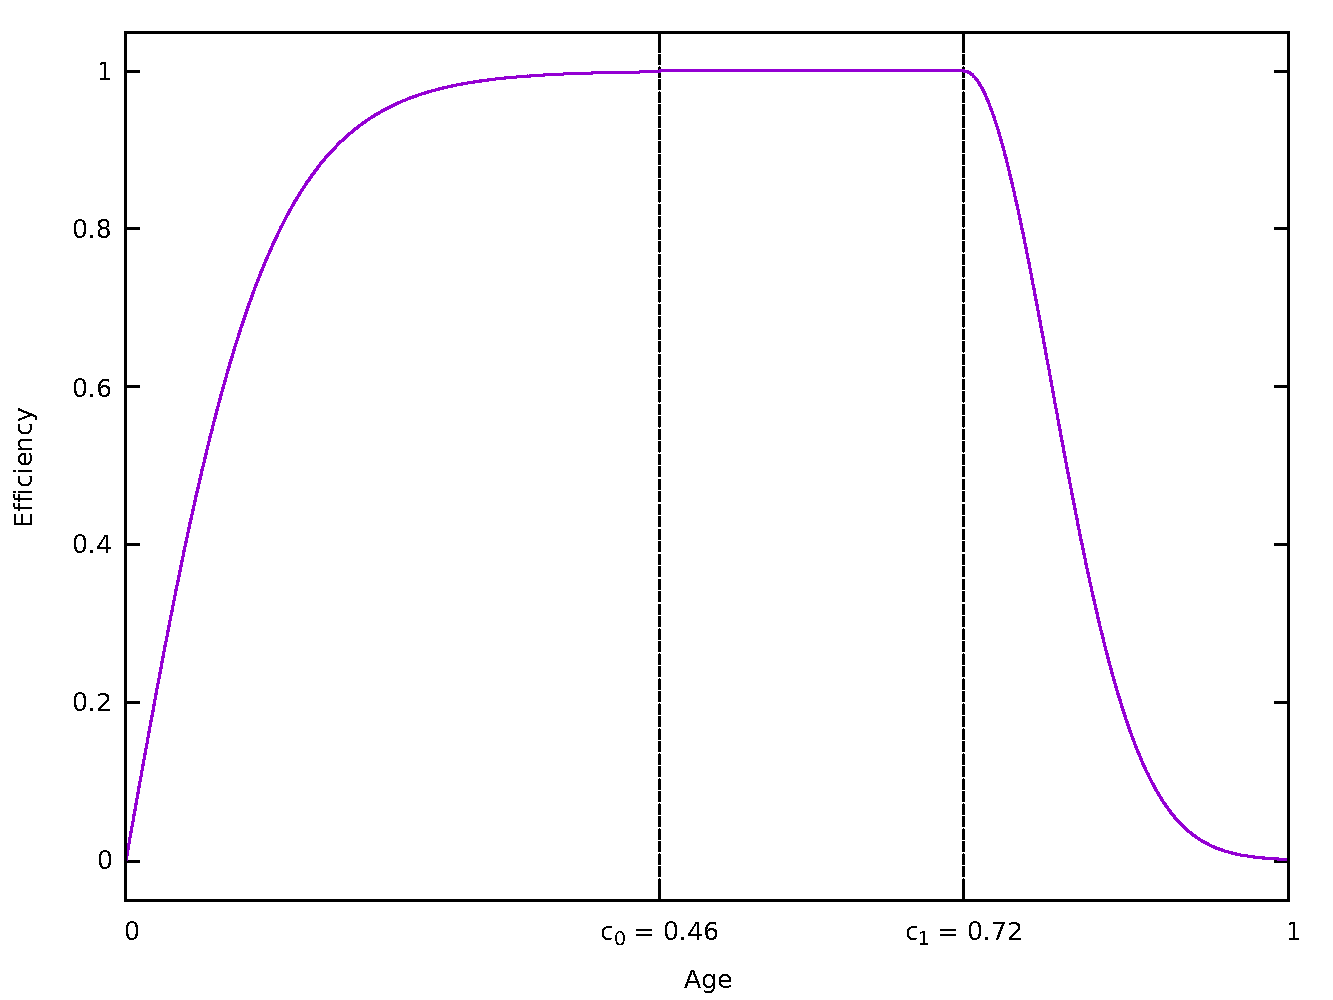
\includegraphics[height=.59\textheight]{efficiency_plot}
 \end{minipage}
 \begin{minipage}{.39\textwidth}
  Age conditions life-step:
  \begin{itemize}
   \item $[0,c_0]$ youth
   \item $[c_0,c_1]$ maturity
   \item $[c_1, 1]$ old age
  \end{itemize}
 \end{minipage}
\end{frame}

\subsubsection{Youth}
\begin{frame}[ok]
 \foreach \i in {0,...,4} {
  \begin{minipage}[c]{.18\textwidth}
   \centering
   \splinoid[scale=.047]{growth_\i}
  \end{minipage}
 }
 \foreach \i in {0,...,4} {
  \begin{minipage}[c]{.18\textwidth}
   \centering\tiny
   \begin{tabular}{c}
    step \i \\
    eff. \pgfmathsetmacro{\e}{100*\i/4}\e \%
   \end{tabular}
  \end{minipage}
 }
 \vfill
 \begin{itemize}
  \item Progressive growth of body size and artifacts
  \item Initial states are highly vulnerable
 \end{itemize}
\end{frame}

\subsubsection{Maturity}
\begin{frame}[ok]
 \begin{itemize}
  \item Reproductive behavior
  \item Based on energy accumulation\footnote{as in \cite{Pichler2008}}
  \item ANN-controlled decision
  \item Not yet implemented
 \end{itemize}
\end{frame}

\subsubsection{Senescence}
\begin{frame}[ok]
  Reduction of maximal speed
  
  > increased chance of starvation and being preyed upon
\end{frame}

\subsection{Sexual dimorphism}
\begin{frame}[ok]
 \begin{minipage}[c]{.49\textwidth}
  \centering \splinoid[scale=.1]{dimorphism_female}
 \end{minipage}
 \begin{minipage}[c]{.49\textwidth}
  \centering \splinoid[scale=.1]{dimorphism_male}
 \end{minipage}
 \vspace{.5\baselineskip}

 \begin{minipage}[c]{.49\textwidth}
  \centering Female
 \end{minipage}
 \begin{minipage}[c]{.49\textwidth}
  \centering Male
 \end{minipage}
 
 \vfill
 Identical genotype (except gender) \\
 $\rightarrow$ different phenotypes (shapes and colors)
\end{frame}

\subsection{Metabolism}
\begin{frame}[ok]
 \begin{itemize}
  \item Energy extracted from plants or corpses
  \item Baseline life cost
  \item Consumed energy returned to the environment
 \end{itemize}
\end{frame}

\subsubsection{Clock speed}
\begin{frame}[ok]
 \begin{itemize}
  \item ANN-controlled value
  \item Genetically controlled bounds 
  \item Impacts:
  \begin{itemize}
   \item Motion speed
   \item Resource absorption
   \item Resource consumption
   \item Regeneration
  \end{itemize}
 \end{itemize}
\end{frame}


\subsection{Neural controller}
\begin{frame}[ok]
 \begin{minipage}{.49\textwidth}
 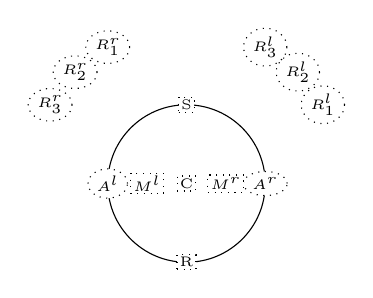
\begin{tikzpicture}[
  nbase/.style={draw, dotted, fill=white, inner sep=1pt, font=\tiny},
  nin/.style={nbase, ellipse},
  nout/.style={nbase}
 ]
  \draw (0,0) circle (1);
  
  \def\p{1}\pgfmathsetmacro{\rs}{2*\p+1}
  \foreach \s/\sl in {-1/l,1/r} {
   \foreach \r in {1,...,\rs} {
    \pgfmathsetmacro{\a}{(\r-1-\p)/\p}
    \node [nin] at (90+\s*45+15*\a:2) {$R^{\sl}_{\r}$};
   }
   \node [nin] at (\s,0) {$A^{\sl}$};
   
   \node [nout] at (.5*\s,0) {$M^\sl$};
  }
  \node at (0,0) [nout] {C};
  \node at (0,1) [nout] {S};
  \node at (0,-1) [nout] {R};
 \end{tikzpicture}
 \end{minipage}
 \begin{minipage}{.49\textwidth}
  \tiny
  \begin{tabular}{r@{: }p{.7\textwidth}}
   \toprule
   \multicolumn{2}{c}{Inputs} \\ \midrule
   $R^s_i$ & retina cell triplet (r,g,b) $i$ on side $s$ \\
   $A^s$   & auditive cells (equal to number of channels) \\
   $-$     & proprioceptors (health, energy, efficiency) \\
   \toprule
   \multicolumn{2}{c}{Outputs} \\ \midrule
     $M^s$ & motor \\
       $C$ & Clock speed \\
       $R$ & Reproduction \\
       $S$ & Multi-channel signal \\
  \end{tabular}
 \end{minipage}
 
 \vfill\centering
 Most nodes are geometrical $\rightarrow$ HyperNeat?
\end{frame}


\section{Environment}
\begin{frame}[ok]
 \centering
 \includegraphics[scale=1.25]{energy_flow}
 
 \vfill
 Closed system with constant total energy level
\end{frame}

\begin{frame}[ok]
 Potential genetic variables:
 \begin{itemize}
  \item Size
  \item Taurus (bool)
  \item Obstacles (distribution)
  \item Plants (distribution)
 \end{itemize}

\end{frame}


\section{Extensions}
\begin{frame}
 \begin{itemize}
  \item Asymetrical offspring investment \\
  $\rightarrow$ Emergence of sexual specialisation?
  \item Day/night cycle \\
  $\rightarrow$ Darkening of colors \\
  $\rightarrow$ Emergence of night-vision? \\
 \end{itemize}

\end{frame}


\setbeamertemplate{frametitle}{}
\doendpages[duration=30 s]{}
% \pageatend

\end{document}
 
